\include{PREAMBLE}

\title{\setstretch{0.9} %will give nice line sep
	\textbf{Little disks operads and configuration spaces}}
\author{Talk by Najib Idrissi \\ 
Notes by Pedro Tamaroff}

\begin{document}
\maketitle

\begin{abstract}
\textbf{Speaker's abstract.} Operads are objects that govern categories of algebras. Initially introduced in the sixties to study iterated loop spaces, they have proved useful in several areas of mathematics. In most of these applications, the little disks operads play a central role. In the first part of this talk, we will focus on one of the applications studied in the 2015 Talbot Workshop, Goodwillie--Weiss embedding calculus, which will serve as an ``excuse'' to introduce operads. In the second part of this talk, I will set out some of the recent developments regarding the links between the little disks operads and the real homotopy types of configuration spaces of manifolds. (Second part based on joint works with Ricardo Campos, Julien Ducoulombier, Pascal Lambrechts, and Thomas Willwacher.)	
\end{abstract}
\bigskip
\tableofcontents

\thispagestyle{frontpage}
%\pagebreak

\section{The embedding calculus}
 
 The motivation to construct the
 embedding calculus on manifolds is 
 the computation of the homotopy type of
 the space $\Emb(M,N)$ of 
 all embeddings $f : M\longrightarrow N$ of one
 manifold into another. Recall that $f$ is
 an \emph{immersion} if its derivative
 $T_pf : T_p M\longrightarrow T_q N$ is 
 injective at each $p\in M$, and it is a (smooth)
 \emph{embedding} if it is an immersion and a 
 topological embedding.
 
 The computation of such space $\Emb(M,N)$ of
 embeddings is highly non-trivial: if $M=S^1$ and 
 $N=S^3$, then the $0$th homotopy group
 $\pi_0\Emb(S^1,S^3)$ consists of all isotopy
 classes of smooth knots, and determining and
 studying these already spans a whole area of
 mathematics, knot theory. 
 
 The fact the previous example is slightly involved
 stems from the fact that the codimension of 
 $S^1$ in $S^3$ is two: as soon as $M$ has
 codimension at least three in $N$, then $\Emb(M,N)$
 is a path connected space. For example, one can
 unknot any embedding $S^1\longrightarrow S^4$.
 Nonetheless, higher homotopy and homology groups
 of $\Emb(M,N)$ are non-trivial, and give interesting
 and fine invariants of $M$ and $N$ that depend on 
 their smooth structure, and not only on
 their homotopy type. 
 
 The immediate problem one encounters when trying
 to compute with the functor $\Emb(-,N)$ is that it
 not continuous (in the categorical sense): if
 $M$ is a union of submanifolds $V\cup U$ then
 $\Emb(M,N)$ is \emph{not} equal to the pullback
 of the cospan
 
 \[
 \begin{tikzcd}
  \Emb(V,N) &  \arrow[r]  \Emb(U\cap V,N)
 \arrow[l]       &  \Emb(U, N).
 \end{tikzcd}
 	 	  	\]
 	 	  	
 Concretely, if one is able to build embeddings
 $V\hookrightarrow N$ and $U\hookrightarrow N$
 that coincide in $V\cap U$,
 it is not always possible to extend them to an
 embedding defined on $M=V\cup U$: the resulting
 map will be an immersion, but may fail to be
 injective on $U\cap V$. 
 
 The idea of Goodwillie--Weiss calculus is to 
 \emph{approximate} the functor $F :M\longmapsto
 \Emb(M,N)$ by a tower of functors
 \[\label{eq:tower} \cdots 
 \longrightarrow F_4 	
 \longrightarrow F_3 	
 \longrightarrow F_2 	
 	\longrightarrow F_1 	
 		\longrightarrow F_0   \] 
 under $F$ that are, in a precise sense, polynomial functors.
 As a first step, one can consider the space of 
 \emph{immersions} $M\longrightarrow N$, which is
 polynomial of order one or, what is the same,
 linear, in the sense that $\Imm(M,N)$ is
 the limit of the span
  \[
 \begin{tikzcd}
  \Imm(V,N) &  \arrow[r]  \Imm(U\cap V,N)
 \arrow[l]       &  \Imm(U, N).
 \end{tikzcd}
 	 	  	\]
 To define what it means for a functor to be ``of
 order at most $k$'' for some $k\in \NN$ requires
 a bit more care, an involves the combinatorics of
 cubical posets. We point the reader to~\cite{}
 for details. The cornerstone of the
 Goodwillie--Weiss calculus is the following 
 result:
 
 \begin{theorem}
 Let $F(V) = \Emb(V,N)$ and suppose that $M$ has codimension
 at least three in $N$. There exists a tower
 of functors over $F$ as in~\eqref{eq:tower} such that the
 map
 \[ F(M) \longrightarrow \operatorname{holim}_k F_k(M)\]
  restricts to a homotopy equivalence of the base
  point components. \textcolor{trinityblue}{Moreover,
  the (homotopy type of the?) functors $F_k(M)$ can be 
  computed in some way using configurations of $k$ points
  of $M$ in $N$. I am not sure how to say this precisely!}\qed
   \end{theorem}
 
  We will in fact take a slightly different approach,
  and use little disks operads and configuration spaces of
  points to obtain a description of the homotopy type of
  $\Emb(M,N)$.
  
 \section{Configuration spaces of points}
  
%  Not the original work of Goodwillie--Weiss but the
% result of a refinement of their work over the years. 
%  Span of maybe two decades. 
  
  We now aim to approximate $\Emb(M,N)$ using
  \emph{configurations spaces}. For each $r\in \NN$,
  we define the \emph{ordered configuration space of
  $r$ points in $M$} by
  \[ \Conf_M(r) = 
  	\{ (x_1,\ldots,x_r)\in M^r 
  	: \text{ $x_i\neq x_j$ for all $i\neq j$} \}. 
  \]
  They appeared initially in the study of braids and
  braid groups by 
  \textcolor{trinityblue}{[I did not get the name]}, 
  and later in the work
  of V. I. Arnol'd~\cite{Arnold1969} and 
  Fadell--Neuwirth~\cite{Fadell1962}.
  Note that,
  more or less by definition, one has
  that the braid group $B_r$ is equal to 
  $\pi_1(\Conf_{D^2}(r))$.
  
 The sequence of spaces $(\Conf_M(r))_{r\geqslant 0}$
 forms a \emph{symmetric sequence} in spaces, that is, 
 it is a sequence of spaces with corresponding actions
 of the symmetric groups, and we will write it $\Conf_M$. 
 They allow us to embed $\Emb(M,N)$ into
 \[ \Map_\Sigma(\Conf_M,\Conf_N) = 
 	\prod_{r\geqslant 0}
 		\hom_{\Sigma_r}(\Conf_M(r),\Conf_N(r))\] 
by assigning an embedding $f:M\longrightarrow N$
to the map $\Phi_f$ that assigns a 
configuration $(x_1,\ldots,x_r)$
in $M$ to the configuration $(f(x_1),\ldots,f(x_r))$. 
There are corresponding constructions
for unframed manifolds. The maps $\Phi_f$ coming from embeddings $f:M\longrightarrow N$
enjoy some additional compatibility properties:
\begin{tenumerate}
	\item \emph{Forgetting points:} the map $\Phi_f$ commutes
	with the maps induced by the forgetful maps 
	$\pi_i : \Conf_M(r) 
	\longrightarrow \Conf_M(r-1)$ that forget the $i$th point
	in the domain. 
	\item \emph{Continuity:} if a configuration $\vec{x_0}$ is
	close to a configuration $\vec{x_1}$ in $M$, then their
	images under $\Phi_f$ will be close as configurations
	in $N$.
	\end{tenumerate}
	
	We would like to relax these two conditions ``up to 
	homotopy''. But what does this mean?
	
	\section{Operads and their modules}
	
	One can use operads to formalize this. Let us consider
	a richer version of configuration spaces, that give us
	some more wiggle room, by replacing points with disks. 
	For each $r\in \NN$, define
	\[ D_m(r) = \Emb_\square(D^m \sqcup \cdots \sqcup D^m , D^m ) \] 
	the space of rectilinear\footnote{We only allow for dilations and translations.} embeddings of $r$ disjoint
	$m$-disks in another $m$-disk. Similarly, define
		\[ D_M(r) = \Emb_\square(D^m \sqcup \cdots \sqcup D^m , M ) \] 
and note that $\Conf_M(r)$ and $D_M(r)$ are homotopy
equivalent spaces. The upshot is that the symmetric sequence
$D_m$ forms a (topological) operad. Namely, it comes equipped
with composition maps
\[ D_m(k)\times D_m(r_1)\times\cdots D_m(r_k) 
	\longrightarrow D_m(r_1+\cdots r_k) \] 
that satisfy certain associativity and equivariance relations.
More briefly, it forms a monoid in the monoidal category of
symmetric sequences under the circle product
\[(X\circ Y)(n) = 
	\bigsqcup_{k\geqslant 0} X(k)\times_{S_k} 
		Y[\lambda], \]
where $Y[\lambda]$ is the $S_k$-module obtained as the
disjoint union of all permutations of $Y(\lambda_1)\times
\cdots \times Y(\lambda_k)$ for $\lambda$ a partition of $n$. With
this at hand, what we want is an equivariant associative map
\[ D_m\circ D_m \longrightarrow D_m. \]
 
 Moreover, the sequence $D_M$ is a right $D_m$-module, in
 the sense there is a map $D_M\circ D_m \longrightarrow D_m$
 that is compatible with the operad structure of $D_m$. 
 Since $n\geqslant m$, there is an inclusion
 of operads $D_m\longrightarrow D_n$, and in particular
 the right $D_n$-module $D_N$ can be viewed as a right
 $D_m$-module, which we will do in what follows.
	
 We now observe that an embedding $f:M\longrightarrow N$
 produces for us a map $D_M \longrightarrow D_N$ that is
 not just a map of symmetric sequences, but in fact a map
 right $D_m$-modules. In this way, it makes sense to form
 the mapping space $\Map_{D_m}(D_M,D_N)$
 and we obtain a map
 \[ \Emb(M,N) \longrightarrow  \Map_{D_m}(D_M,D_N)\] 
 by virtue of the additional compatibility properties we
 observed before. With this at hand, we can state
 the following theorem:
 
 \begin{theorem}[Goodwillie--Weiss, Arone--Turchin, Turchin, Boavida--Weiss, Sinha, ...] If $M$ has codimension at least
 three in $N$, then the map above induces a homotopy
 equivalence
 \[ \label{eq:derivedMap}
 	\Emb(M,N) \longrightarrow \mathbb R \Map_{D_m}(D_M,D_N)\]
 where the right hand side is the \emph{derived}\footnote{For 
 details, the reader can consult the work of B. Fresse~\cite{}.} 
 mapping space of $D_m$-module maps $D_M\longrightarrow D_N$.
 \qed
  \end{theorem}
 
 It is useful to note that the derived mapping space describes the
 ``$F_\infty$ term'' in the Goodwillie--Weiss tower for
 $\Emb(M,N)$, and that one can use truncated versions of
 mapping spaces to describe the finite stages of the tower.
 
 The upshot of this result is that if we can understand
 the homotopy type of the configuration spaces as right
 modules over the little disk operad, then we can understand
 the homotopy type of the space of embeddings. However,
 there is a 
 trade-off: we now need to determine the homotopy type of
 a very simple manifold into another ---a disjoint union of
 points--- but nonetheless the functor 
 $M\longmapsto \Conf_M(r)$ is not
 easy to compute. In particular, it is not homotopy
 invariant! For example, the point has empty higher
 configuration spaces, but the contractible space
 $D^2$ has $\Conf_{D^2}(2) \simeq S^1$. More
 generally, $\Conf_{D^m}(2)$ is homotopy equivalent
 to $S^{m-1}$, through the map
 \[ (v,w) \longmapsto \frac{v-w}{|v-w|}.\] 
 
 One may suspect that the problem above is that the
 manifold $D^2$ is not closed (compact), 
 but Longoni--Salvatore~\cite{}
 have proved that the lens spaces $L_{7,1}$ and $L_{7,2}$,
 which are homotopy equivalent, have non-homotopy
 equivalent configuration spaces. However, these 
 are non-simply connected spaces, and the following
 is still an open question:
 
 \begin{question*}
 Is it true that two simply connected closed manifolds
 of the same homotopy type have homotopy equivalent
 configuration spaces?
 \end{question*}
 
 
 \subsection{Bonus: deloopings}
 
 The little disks operads were initially introduced to
 study and identify when a space can be delooped. That is,
 given a space $X$, when is it weakly homotopy equivalent
 to a space of the form
 \[ \Omega^n(Y) = \Map(D^n;S^{n-1}, Y;\ast) \] 
 for some other space $Y$? Any loop space $X=\Omega Y$ is an $H$-space and, as such,
 the monoid $\pi_0(X)$ is in fact group like, in the sense
 it is a group under the induced product of $X$. Moreover,
 it is an algebra over the little $n$-disks operad: there
 are equivariant maps
 $D_n(k) \times X^k \longrightarrow X$
 obtained by inserting maps $D^n\longrightarrow Y$
 into a disk configuration to obtain a new map 
 $D^n\longrightarrow Y$, which is associative in a precise
 sense.\footnote{Which one?}
 
 Conversely, one can consider such a $D_n$-algebra $X$
 which, in particular, comes equipped with a single
 homotopy class of operations $m: X^2\longrightarrow X$
 originating from $\pi_0(D_n(2))$, making $\pi_0(X)$
 into an associative monoid. We say $X$ is a \emph{group-like}
 $D_n$-algebra if this monoid is in fact a group.
 
 With this at
 hand, we can state the following result, going back to work
 of Beck, Boardman-Vogt, May, Segal and Stasheff. The
 theorem, due to J. P. May~\cite{}, provides a useful theorem to
 determine when a space can be delooped.
  
 \begin{theorem} A space $X$ is weakly equivalent to
 an $n$th loop space $\Omega^n(Y)$ if, and only if,
 it is a group-like $D_n$-algebra.  \qed
 \end{theorem}
 
 \section{The homotopy type of configuration spaces}
 
 Computing integral homotopy types of spaces and, in particular,
 of configuration spaces, is remarkably difficult. A useful simplification
 that still allows us to obtain significant information on the
 homotopy type of a space is to work rationally. Informally, one
 can think that we are throwing away the torsion of homotopy groups
 of a space. 
 
 More precisely, a simply connected topological space $X$ is
 \emph{rational} if all of the abelian groups $\pi_n(X)$
 for $n\geqslant 2$ are $\mathbb Q$-vector spaces. A map of
 spaces $f:X\longrightarrow Y$ is a \emph{rationalization}
 if $Y$ is a rational space and the induced map $\pi_*(X)\otimes \mathbb Q \longrightarrow \pi_*(Y)$ is an isomorphism. One can show such
 space $Y$ is unique up to homotopy equivalence relative to $X$,
 and we write it $X_{\mathbb Q}$.
 
 We say $f$ is a
 \emph{rational homotopy equivalence} if the following
 equivalent conditions hold:
 \begin{tenumerate}
 \item The map $\pi_*(f)\otimes \mathbb Q$ is an isomorphism.
 \item The map $H_*(f,\mathbb Q)$ is an isomorphism.
 \item The map $H^*(f,\mathbb Q)$ is an isomorphism.
 \end{tenumerate} 
 We call the weak homotopy type of $X_{\mathbb Q}$ the \emph{rational
 homotopy type of $X$}. For example, the odd sphere $S^{2n+1}$ have
 the rational homotopy type of a $K(2n+1,\mathbb Q)$, while
 the even sphere have a slightly (but still simple) rational
 homotopy type.  
 In this sense, doing homotopy theory over
 $\mathbb Q$ is much simpler, at the cost of losing some
 information (for example, torsion, Steenrod operations, among
 others). The following theorem is one of the cornerstones of 
 rational homotopy theory, along with the seminal work of 
 D. Quillen~\cite{}:
 
 \newcommand\rightleftarrow{%
        \mathrel{\vcenter{\mathsurround0pt
                \ialign{##\crcr
                        \noalign{\nointerlineskip}$\longrightarrow$\crcr
                        \noalign{\nointerlineskip}$\longleftarrow$\crcr
                 }%
        }}%
}

 \begin{theorem}[Sullivan] There is a Quillen adjunction\footnote{A special kind of adjunction, see~\cite{RHT} for details.}
 \[ \Omega^*(-) : \mathsf{Top}^{\geqslant 1} 	
  \rightleftarrow \mathsf{CDGA}^{\geqslant 1} : \langle -\rangle\] 
 between the category of simply connected\footnote{There is a corresponding theory for non-simply connected spaces
 that require nilpotence hypotheses on fundamental groups.
} topological spaces of
 finite type up to rational equivalences and
 simply connected commutative dg algebras of finite type up to
 quasi-isomorphism. \qed
 \end{theorem}
 
 The functor $\Omega^*(X)$ is analogous to the de Rham functor of
 forms, but instead consists of `piece-wise linear polynomial forms'
 on $X$, while the functor $\langle A\rangle$ is a `geometric realization'
 functor. The upshot of this theorem is that the determination of the
 rational homotopy type of a space $X$ is a purely algebraic task,
 and can be done by producing a cdga model of the (non-commutative)
 dga of cochains $C^*(X)$. For example, for each $n\geqslant 1$ 
 the free commutative algebra $(S(x_{2n+1}),0)$ on a single generator 
 of degree $2n+1$ is a model for the rational homotopy type of the
 odd sphere $S^{2n+1}$, 
 while the commutative algebra $(S(x_{2n},y_{4n-1}),d)$ with
 $dy_{4n-1} = x_{2n}^2$ is a model for the rational homotopy
 type of the even sphere $S^{2n}$. 
 
 The end goal of rational homotopy theory is reproducing such
 computation for more complicated spaces or, what is the same,
 solving the following problem: given a space $X$, determine
 a cdga $A^*(X)$ that is `nice enough' and quasi-isomorphic
 to the cdga of PL-forms $\Omega^*(X)$. The model $A^*(X)$
 will then give us information about the rational homotopy
 type of $X$. For example, if $A^*(X)$ is minimal, in the sense
 that $A^*(X) = (S^*(V),d)$ with $dV \subseteq S(V)^{\geqslant 2}$,
 then $V^* \cong \hom_{\mathbb Q}(\pi_*(X),\mathbb Q)$.
 
 \emph{Back to operads and modules.} With this at hand, our goal is
 to find a model for $\Omega^*(D_m)$ and $\Omega^*(D_M)$, taking into
 account that the former is (almost) a cooperad ---the functor 
 $\Omega^*$ is  contravariant--- and latter is a comodule over it.
 Since $\Omega^*$ is a good functor, these models will allow us to
 compute the derived mapping space in~\eqref{eq:derivedMap}, at least
 rationally, ultimately allowing us to pin down the rational homotopy
 type of $\Emb(M,N)$. 
 
 \subsection{The case of Euclidean space}
 
 Let us begin with the case $M=\mathbb R^m$, the building block
 for any other $m$-manifold. In this case, the computation of the
 cohomology groups of $\Conf_M(r)$ for all $r\geqslant 1$ are well
 understood and date back to work of V. I. Arnol'd and F. Cohen.
 For each $r$ and each distinct $i,j\in [r]$, there is a map
 \[ \Conf_M(r) \longrightarrow \Conf_M(2) \simeq S^{m-1} \]
 that produces for us a cohomology class of degree $m-1$ that
 we write $\omega_{ij}$. Note that exchanging $i$ and $j$ 
 induces the antipodal map on $S^{m-1}$, creating a $(-1)^m$
 sign for this cohomology class. Coming from the top cohomology
 class of the sphere, $\omega_{ij}^2=0$ and, by looking at
 configurations
 of three points, one arrives at the following `Jacobi-like
 identity' for three distinct $i,j,k\in [r]$:
 \[ \label{eq:Jacobi} 
 	\omega_{ij}\omega_{jk}
 		 + \omega_{jk}\omega_{ki} 
 	 		+ \omega_{ki}\omega_{ij} = 0. \]
 These is in fact a complete presentation of $H^*(D_m(r),\mathbb Q)$:
 \begin{theorem}[Arnol'd, Cohen]
 The cohomology ring $H^*(D_m(r),\mathbb Q)$ is isomorphic to the
 commutative algebra generated by $\omega_{ij}$ in degree $m-1$
 for $i,j\in [r]$ subject to the following three sets of relations:
 \begin{enumerate}[label=$R_{\arabic*}$:]
  \setlength{\itemsep}{0pt}
  \setlength{\parskip}{0pt}
 \item For all distinct $i,j$ we have that $\omega_{ij} = (-1)^m \omega_{ji}$.
 \item For all distinct $i,j$ we have that $\omega_{ij}^2 =0$.
 \item For all distinct $i,j,k$ we have the Jacobi relation~\eqref{eq:Jacobi}.
 \end{enumerate}
 \end{theorem}
 
 In fact, Cohen computed the cooperadic decomposition maps of
 $H^*(D_m(r),\mathbb Q)$, thus determining it completely as a
 Hopf cooperad: the operad $H_*(D_m,\mathbb Q)$ is isomorphic
 to the operad of Poisson algebras with a commutative product
 of degree zero and a Lie bracket of degree $m-1$\footnote{Integrally, the description of the algebras governed by the homology of configuration spaces is much more complicated.}.
 In general, this computation would not be enough to determine
 the rational homotopy type of $D_m$. However, the following
 formality result says that indeed this cohomology ring is
 quasi-isomorphic to the algebra of forms $\Omega^*(D_m)$,
 and thus does capture the rational homotopy type of $D_m$:
 
 \begin{theorem}[Kontsevich, Lambrechts--Voli\'c, Tamarkin,...]
 The operad $D_m$ is formal: there are quasi-isomorphisms
 of Hopf cooperads
 \[ \label{eq:formality}
 	 H^*(D_m) \longleftarrow \cdot 
 	 	\longrightarrow \Omega^*(D_m). \] 
 \end{theorem}
 
 At the time, results on various flavour of formality of the operad
 $D_m$ abound, see~\cite{Fresse2018, Petersen2013, Tamarkin2003, BoavidadeBrito2021}. One of 
 the two most famous consequences of formality of $D_2$ are the 
 solution of the Deligne conjecture (for example, as was done by
 Tamarkin and explained in~\cite{Hinich2003}) and the deformation quantization
 theorem of Kontsevich~\cite{}. 
 For us, formality has the consequence of 
 allowing us to restrict to cohomology when computing our derived
 mapping space of interest. 
 
 \subsection{Two approaches to formality}
 
 \textsc{Kontsevich's approach} 
 to obtaining the formality result in the last
 theorem can be summarized as follows. First, one can find `arity
 wise' resolutions of the commutative algebras $H^*(D_m(r))$, which
 involve, for example, introducing a new generator $\xi_{ijk}$ 
 relaxing the Jacobi identity of~\eqref{eq:Jacobi} up to homotopy:
 \[ d\xi_{ijk} = \omega_{ij}\omega_{jk}
 		 + \omega_{jk}\omega_{ki} 
 	 		+ \omega_{ki}\omega_{ij}. \] 
 If we interpret $\omega_{ij}\omega_{jk}$ as the directed  graph
 (and interpret the other two terms similarly)
 
 \tikzset{>=latex}
\[
 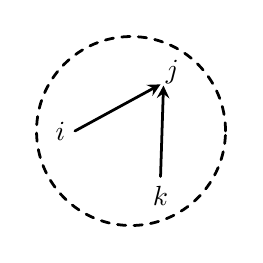
\begin{tikzpicture}[line cap=round,line join=round,x=1.0cm,y=1.0cm, scale = .75]
\clip(-1.75,-1.75) rectangle (1.75,1.75);
\draw [line width=1.pt,dash pattern=on 3pt off 3pt] (0.,0.) circle (1.6 cm);
\draw [->,>=stealth,line width=1.pt] (-0.95,0) -- (0.5,0.79);
\draw [->,>=stealth,line width=1.pt] (0.5,-0.77) -- (0.55,0.77);
\draw (-0.95,0.0) node[anchor=east] {$i$};
\draw (0.7,1) node {$j$};
\draw (0.5,-0.77) node[anchor=north ] {$k$};
\end{tikzpicture}
	\]

then we may interpret $\xi_{ijk}$ as the directed
graph 

\[
 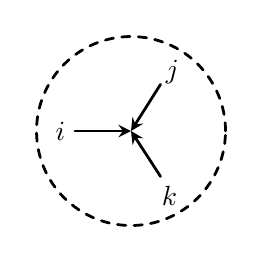
\begin{tikzpicture}[line cap=round,line join=round,x=1.0cm,y=1.0cm, scale = .75]
\clip(-1.75,-1.75) rectangle (1.75,1.75);
\draw [line width=1.pt,dash pattern=on 3pt off 3pt] (0.,0.) circle (1.6 cm);
\draw [->,>=stealth,line width=1.pt] (-0.95,0) -- (0,0);
\draw [->,>=stealth,line width=1.pt] (0.5,0.79) -- (0,0);
\draw [->,>=stealth,line width=1.pt] (0.5,-0.77) -- (0,0);
\draw (-0.95,0.0) node[anchor=east] {$i$};
\draw (0.7,1) node {$j$};
\draw (0.65,-0.77) node[anchor=north ] {$k$};
\end{tikzpicture}
	\]

with differential the Jacobi relation, obtained by
contracting one edge at a time. This idea gives rise
to an object called a graph complex, filling in the
`dot' in~\eqref{eq:formality}. The map pointing to the
left is obtained by assigning an integral 
to each labeled graph with some internal (black) vertices,
and giving rise to an element in $\Omega^*(D_m)$.
For details, the reader can refer to the book of
Lambrechts and Voli\'c~\cite{LambrechtsVolic2014}.

It is worth pointing out that one can show the
framed little disks operad $D_2^{\mathrm{fr}}$
is formal, this was done by Giansiracusa--Salvatore~\cite{}.
Later, S. Moriya~\cite{} and Turchin--Willwacher~\cite{} showed that
the framed little disks operad $D_{2m+1}^{\mathrm{fr}}$ is
not formal for $m\geqslant 2$.

\textsc{Tamarkin's approach}, on the other hand, can be
summarized as follows. There is an operad in groupoids called the
\emph{parenthesized braids operad}, which we write
$\mathsf{PaB}$\footnote{Following Tamarkin's original notation.}. 
The elements of $\mathsf{PaB}$ are
parenthesized permutations $(\sigma,\pi)$
of some finite set $[r]$, and the morphisms between
$(\sigma,\pi)$ and $(\sigma',\pi')$ consist of the
elements of $B_r$ that join an element in $\sigma$
with the same element in $\sigma'$, as in Figure~\ref{fig:braids}
below. Tamarkin's observation is that the geometrical
realization of this operad in groupoids is \emph{a} little disks
operad ---what is now called an $E_2$-operad--- and that
to show $D_2$ is formal, it suffices to show his
operad of parenthesized braids is formal: any two pair
of $E_2$-operads are connected by a zig-zag of quasi-isomorphisms,
so this suffices.
 	 
 	 \begin{figure}
 	 \begin{center}
 	 	\includegraphics[scale=.15]{braids.png}
 	 \end{center}
 	 	\caption{The generators of $\mathsf{PaB}$.}
 	 \label{fig:braids}
 	 \end{figure}
 	 
It is well known that each topological
space $D_2(r)$ is a $K(PB_r,1)$ where $PB_r$ is the pure braid 
group on $r$ strands. For Tamarkin, a topological $B_\infty$-operad
is a topological operad $X$ where each $X(r)$ is a contractible
space carrying a free action of the braid group $B_r$. The
corresponding little disks operad is $E_2(X) = X/PB$, the
arity-wise quotient of $X(r)$ by $PB_r$\footnote{Note that $B_r/PB_r = S_r$, so we get a symmetric operad.}. Naturally, $D_2$
is the associated $E_2$-operad of its classifying space.
 
To show that $\mathsf{PaB}$ is formal, Tamarkin shows that
every Drinfel'd associator produces a map of Hopf operads from
$C_*(\mathsf{PaB})$ to the Chevalley--Eilenberg complex 
$\mathscr{C}_*(\mathfrak{t})$ of the Drinfel'd--Kohno
Lie algebras~\cite{}
\[ \mathfrak{t} = ( \mathfrak{t}_1,\mathfrak{t}_2,\mathfrak{t}_3,\ldots)\]
which form an operad in Lie algebras.
Since these are the Koszul dual Lie algebras to the
commutative model of Arnol'd and Cohen, this
produces for the requisite quasi-isomorphisms,
and thus shows that every $E_2$-operad is formal.
Thus, Tamarkin's result can be stated as follows:

\begin{theorem}[Tamarkin]
The $E_2$-operad of parenthesized braids $\mathsf{PaB}$ is
formal, and each Drinfel'd associator $\Phi$ produces a quasi-isomorphism
of Hopf operads 
\[ f_\Phi: C_*(\mathsf{PaB}) 
	\longrightarrow \mathscr{C}_*(\mathfrak{t})\]
where the right hand side is the Chevalley--Eilenberg 
construction of the Drinfel'd--Kohno Lie algebras,
which receives a quasi-isomorphism
\[ H_*(D_2) \longrightarrow \mathscr{C}_*(\mathfrak{t}).\] 
\end{theorem}

It is worth to note that proving Koszulness of the 
commutative algebras $H^*(D_m(r))$ or, equivalently,
of the Lie algebras of Drinfel'd--Kohno, is a highly
not trivial task.

Later, \u{S}evera showed that the operad $D_2^{\mathrm{fr}}$
of \emph{framed} little disks is formal. This operad is isomorphic
to $D_2(r)\times (S_1)^r$ in each arity: each disk in a little
disks configuration is now given a framing, that is, a point
in its boundary is marked. The operad  $D_2^{\mathrm{fr}}$ is
\emph{cyclic}, in the sense that the $S_r$ action on
 $D_2^{\mathrm{fr}}(r)$ extends to an $S_{r+1}$ action (the
 output is now no longer `special') along with a compatibility
 condition with the composition maps, and one can consider
 the problem of formality of $D_2^{\mathrm{fr}}$ as a 
 cyclic operad. Inspired by \u{S}evera's proof, we have
 the following result:
 
 \begin{theorem}[Campos--Idrissi--Willwacher~\cite{}] The
 cyclic operad $D_2^{\mathrm{fr}}$  is formal. \qed
\end{theorem}  

\subsection{Configuration spaces of closed manifolds}

Let us fix a closed manifold $M$, and consider the problem
of determining the homotopy type of $\Conf_M(r)$ for a fixed
$r$. If we expect it possible to obtain the homotopy type
of $\Conf_M(r)$ from that of $M$, it makes sense to consider
a mode $A$ of the space $\Omega^*(M)$ of PL-forms on $M$,
and attempt to build a model of $\Conf_M(r)$ out of $A$.

One can in fact do this over the reals. Let us define
$G_A(r)$ to be the cdga obtained from $A^{\otimes r}$ ---or,
what is the same, a model of $M^r$---
by adding generators $\omega_{ij}$ for distinct $i,j\in [r]$
that satisfy the three sets of Arnol'd relations, along
with the two additional sets of relations:
 \begin{enumerate}[label=$S_{\arabic*}$:]
  \setlength{\itemsep}{0pt}
  \setlength{\parskip}{0pt}
 \item (Symmetry) For each $i,j\in [r]$ and each $x\in A$
 we have that $x_i\omega_{ij} = x_k\omega_{ij}$, where
 $x_i$ corresponds to the copy of $x\in A$ in the $i$th
 factor of $A^{\otimes r}$.
 \item (Killing the diagonals) For each $i,j\in [r]$
 we have that $d\omega_{ij} = [\Delta_{ij}]$, the class
 of the thick diagonal in $M^r$.
 \end{enumerate}
 
 We call $G_A(r)$ the \emph{Lambrechts--Stanley model of
 $\Conf_M(r)$}, as it was conjectured by these authors that
 $A(r)$ does provide us with such a model. This conjecture
 was confirmed over the reals:
 
 \begin{theorem}[Idrissi~\cite{}]
 For each closed manifold $M$ of dimension at least four
 and each model $A$ of $M$,
 the Lambrechts--Stanley cdga $G_A(r)$ is a model of
 $\Conf_M(r)$ over $\mathbb R$. In particular,
 the real homotopy type of $\Conf_M(r)$ depends only
 on the real homotopy type of $M$. \qed
 \end{theorem}
 
 In related work, Campos--Willwacher obtain a description
 of a model of $\Conf_M(r)$ over $\mathbb R$, thus obtaining
 an independent proof of real homotopy invariance of
 configuration spaces for closed manifolds. Later, in
 joint work, Campos--Idrissi--Willwacher obtain a small
 model for the framed configuration space of a compact
 surface of genus $g$.
 
 Concretely, let us fix a compact surface $\Sigma_g$ of genus $g$,
 and let us write $\alpha_1,\ldots,\alpha_g,\beta_1,\ldots,\beta_g$ 
 for the canonical generators of $H^*(\Sigma_g)$. Let us write
 $\theta$ for the Thom class of $\Sigma_g$ and, in addition to the
 relations we wrote before, let us add the 
 relations that:
  \begin{enumerate}[resume, label=$S_{\arabic*}$:]
  \setlength{\itemsep}{0pt}
  \setlength{\parskip}{0pt}
 \item (Thom class) For each $i \in [r]$ we have
 that $d\theta_i = (2-2g)\cdot \mathrm{Vol}_i$, the volume
 form corresponding to the $i$th copy of $\Sigma_g$.
 \item (Volume form) For each $i,j\in [g]$ and each
 $k\in [r]$ we have that 
 $\alpha_{i,k}\beta_{i,k} = \alpha_{j,k}\beta_{j,k}$. 
 \textcolor{trinityblue}{I do not think I understood
 what `and zero otherwise' means.}
 \end{enumerate}
 Remark that the relations that hold in $A$ (the canonical model
 of $\Sigma_g$) are implicit throughout. Let us write this
 model $G_{\Sigma_g}^\mathrm{fr}(r)$. With this at hand, we
 have the following result:
 
 \begin{theorem}[Campos--Idrissi--Willwacher~\cite{}] 
 The Hopf cooperad $G_{\Sigma_g}^\mathrm{fr}$ is a 
 real model of $D_{\Sigma_g}^{\mathrm{fr}}$.
 \end{theorem}

 
 \pagebreak
 
 
 
\bibliographystyle{alpha}
\bibliography{biblio}


\Addresses

\end{document}
